\documentclass[11pt]{standalone}
\usepackage{tikz}

\usetikzlibrary{calc}
\begin{document}
\begin{tikzpicture}
    % Include the image in a node
    \node[anchor=south west, inner sep=0] (image) at (0,0) {
        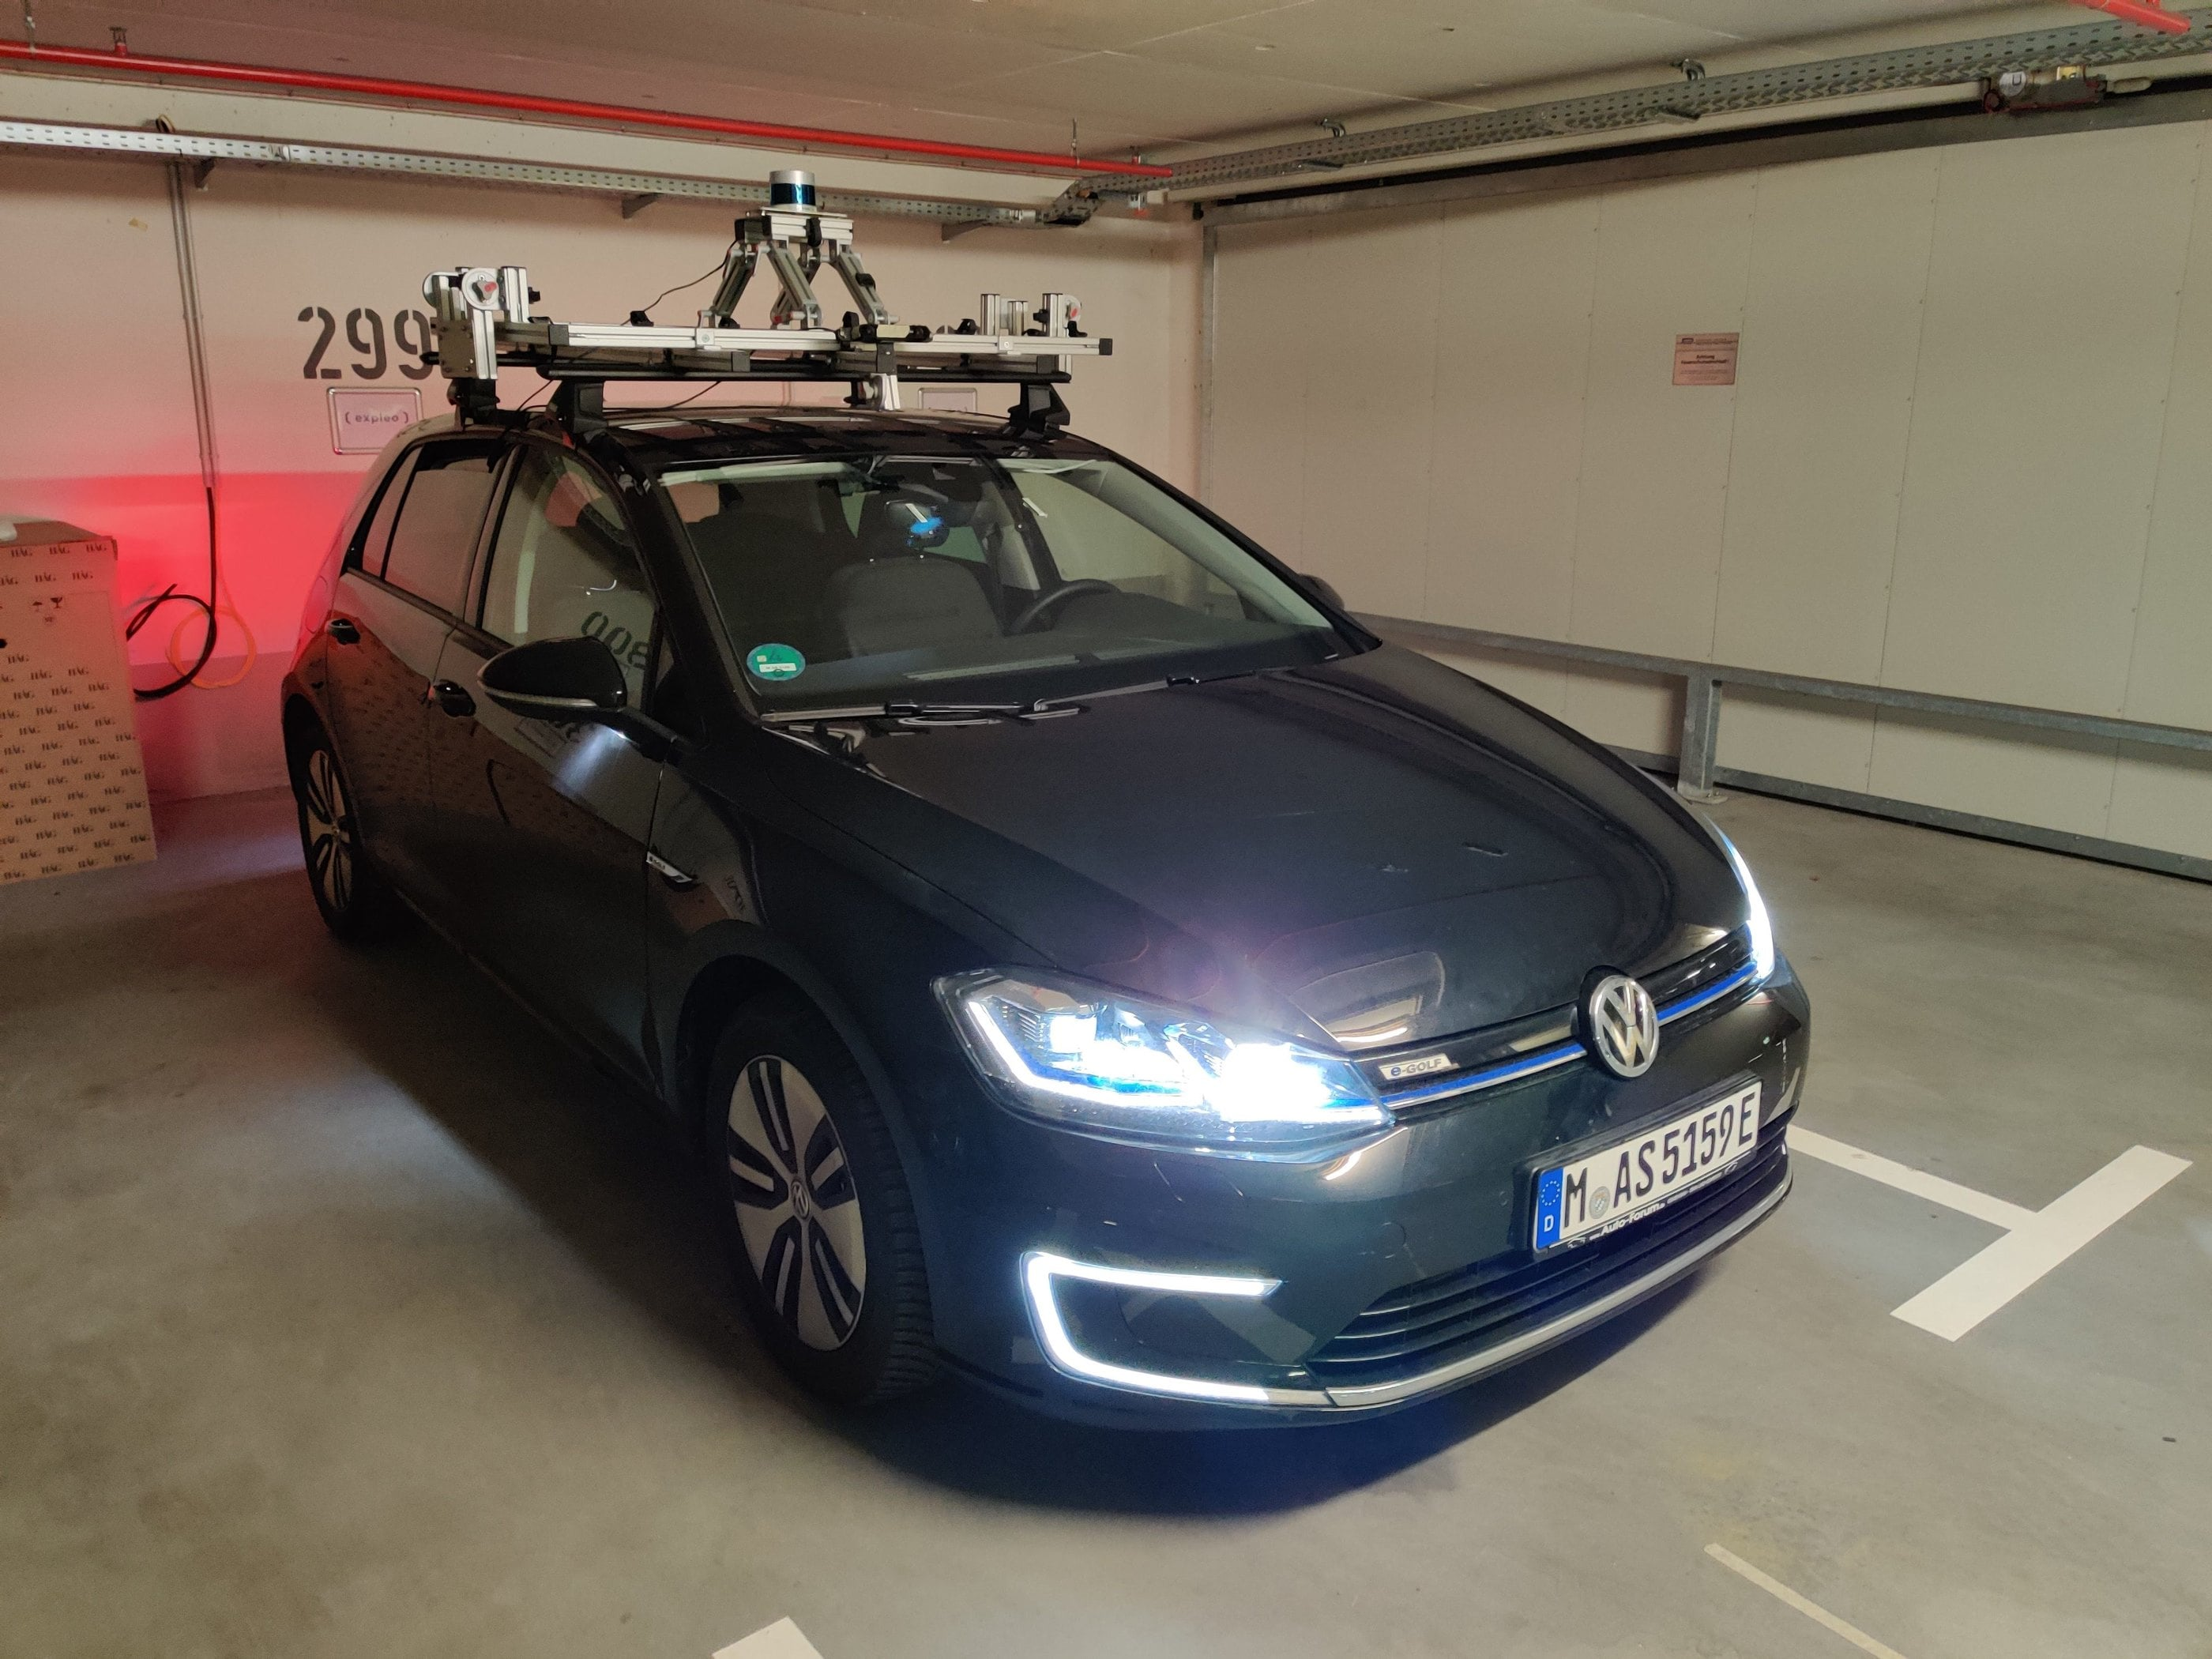
\includegraphics[trim={0, 5cm, 0, 3cm}, clip, width=0.6\textwidth]{eGolf}
    };

    % Create scope with normalized axes
    \begin{scope}[
            x={($0.1*(image.south east)$)},
            y={($0.1*(image.north west)$)}]

        % % Grid (for easier positioning of nodes)
        % \draw[lightgray,step=1] (image.south west) grid (image.north east);
        % % Axes' labels
        % \foreach \x in {0,1,...,10} { \node [below] at (\x,0) {\x}; }
        % \foreach \y in {0,1,...,10} { \node [left] at (0,\y) {\y};}

        % Labels
        \draw[latex-, green] (3.9,9.1) -- ++(2.5,0)
        node[right,black,fill=white, rounded corners=.07cm]{\small LiDAR};
        \draw[latex-, green] (4.3,8.2) -- ++(2.1,-.7)
        node[right,black,fill=white, rounded corners=.07cm]{\small Camera};


        \draw[green] (3.3,8.7) rectangle (3.9,9.5);
        % node[below left,black,]{1};
        \draw[green] (3.7,8) rectangle (4.3,8.4);
        % \draw[very thick,green] (3.3,8.7) rectangle (3.9,9.5);
    \end{scope}

\end{tikzpicture}
\end{document}